% !TeX root = ../../main.tex
% Add the above to each chapter to make compiling the PDF easier in some editors.

\section{Polygon Drawing}\label{ord:ch3:sec1}

In contrast to the previously introduced interactive segmentation approaches, this manual polygon drawing acts as baseline without the use of intelligent or clever algorithms.
A polygon is created by using mouse clicks to set points in the image.
From three points on a polygon is spanned, where each point functions as a node.
% Each point has two edges.
To label an object in an image the points are set on the border of the object and the area inside the polygon represents the object mask as shown in Figure \ref{fig:ch3:sec1:polygon_method}.

There are two ways to set points.
First, to set one point after another by one mouse click for each point.
Second, to draw multiple points by moving the mouse, this also referred to as \textit{stroke}.
This is done by pressing the left mouse button, moving the mouse and releasing the left mouse button.
On the drawn way multiple points with a certain spacing are set.

Further, there are additional features implemented, in order to facilitate the drawing process.
Each new set point is automatically included into the nearest edge of the polygon.
Set points can be relocated by a functionality similar to \textit{drag and drop}.
A set point can be removed by dragging it into a neighboring point, such that only one point remains.
There is the possibility to create holes by drawing a hole-polygon into an existing annotation.

This polygon drawing method is included in the benchmark study in order to evaluate the other methods to a baseline, which represents mostly manual drawing.

\begin{figure} [h]
	\centering
	\begin{subfigure}[t]{0.45\textwidth}
		\centering
		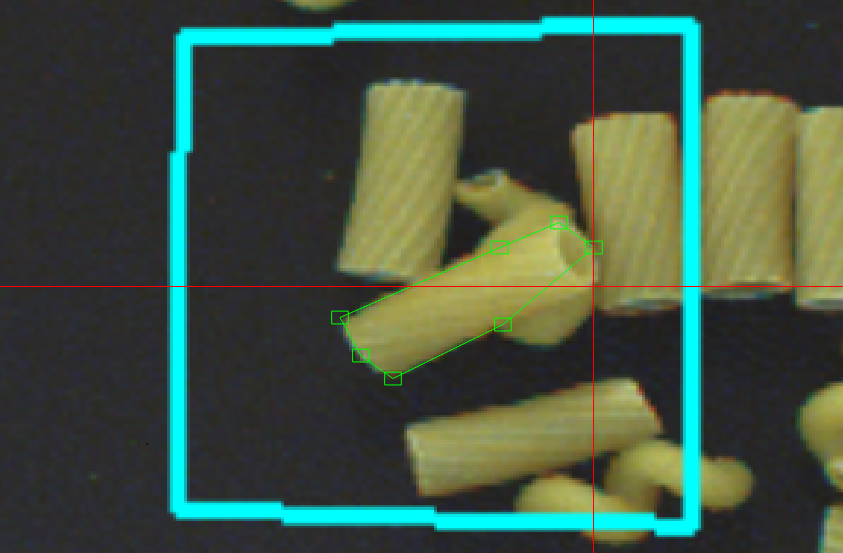
\includegraphics[width=\textwidth]{figures/chap31_polygon_drawing.png}
		\caption{
			Process of drawing a polygon by setting several points.
			The points (visualized as green boxes) are set by mouse clicks and the red crosshair serves as assistance.
		}\label{fig:ch3:sec1:polygon_drawing}
	\end{subfigure}
	\hfill
	\begin{subfigure}[t]{0.45\textwidth}
		\centering
		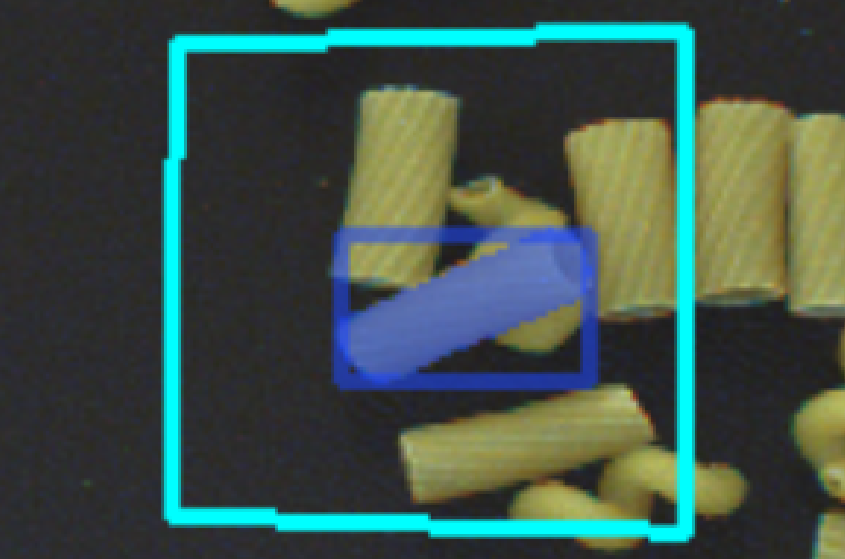
\includegraphics[width=\textwidth]{figures/chap31_polygon_result.png}
		\caption{
			The result after finishing drawing the polygon is the object mask (in blue) and the corresponding bounding box.
			The surrounding turquoise polygon defines the label region.
		}\label{fig:ch3:sec1:polygon_result}
	\end{subfigure}
	\caption[Illustration of the polygon method]{
		Illustration of the polygon method as baseline as for the benchmark study.
	}\label{fig:ch3:sec1:polygon_method}
\end{figure}
